\chapter{Mini Case-Study}
\label{chapter:MiniCaseStudy}
This chapter provides a mini case-study evaluating the developed recovery system for this thesis.
§\ref{section:ExampleCorpus} outlines the corpus used for evaluation.
§\ref{section:Metrics} describes metrics used to evaluate the system.
§\ref{section:Results} discusses results of the case-study.

\section{Corpus}
\label{section:ExampleCorpus}
The example corpus used to evaluate the recovery system for this thesis consists of artifacts implementing a fictional \gls{HRMS} within an \gls{O/R/X-Mapping} scenario using \gls{Java} technologies.
The model is provided by the 101wiki\footnote{\url{https://101wiki.softlang.org/} (retrieved \formatdate{12}{11}{2017})}, where it is used for contributions.
It is implemented using plain \Gls{Java} and then mapped to plain \gls{XML}/\gls{XSD} with \gls{JAXB} and to \gls{SQL/DDL} statements using \gls{Hibernate} mapping files and/or annotations.



\subsection{The 101HRMS Model}
\gls{101HRMS}\footnote{\url{https://101wiki.softlang.org/101:@system} (retrieved \formatdate{12}{11}{2017})} provides a simple model of a company with many departments and employees.
Figure \ref{figure:101HRMSModel} shows an \gls{UML} class diagram of a variant of this model.

\begin{figure}[h!]
\begin{center}
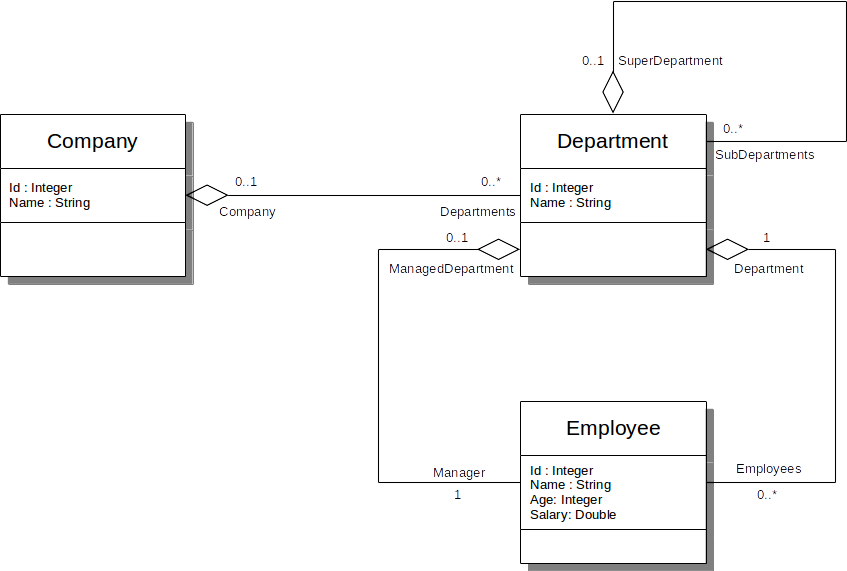
\includegraphics[scale=.5]{images/101HRMSModel.png}
\end{center}
{
\scriptsize 
This \gls{UML} class diagram depicts the model of the \gls{101HRMS}.
It consists of simple companies with nested departments and employees mapped to the latter.
}
\caption{The 101 Human Resource Management System Model}
\label{figure:101HRMSModel}
\end{figure}

The \gls{101HRMS} model consists of companies attributed with a name.
Each company accumulates departments.
Each department is also attributed with a name, aggregates employees and has one employee acting as manager.
Departments can further be refined into sub-departments.
Each employee is attributed with a name, an age and a salary.
Each entity is also attributed with an ID.

\subsection{Linguistic Domains of the Example Corpus}
The example corpus used to evaluate the recovery system contains artifacts implementing the \gls{101HRMS} model generated or used by \gls{Java} technologies for \gls{O/R/X-Mapping}, i.e. a \gls{Java} model is mapped to plain \gls{XML}/\gls{XSD} with \gls{JAXB}, to a \gls{Hibernate} mapping file and to \gls{SQL}/\gls{DDL} statements.
Figure \ref{figure:ExampleCorpusJORXDomains} shows a schematic illustration of the linguistic domains involved:
\begin{description}

\item[Java]
The language and technology used to implement the \gls{101HRMS} model.

\item[XML]
The language used to serialize the \gls{101HRMS} model.

\item[SQL/DDL]
The language used to persist the \gls{101HRMS} model.

\item[JAXB]
The technology used to implement \gls{O/X-Mapping} of the \gls{101HRMS} model.

\item[Hibernate]
The technology used to implement \gls{O/R-Mapping} of the \gls{101HRMS} model.

\end{description}

\begin{figure}[h!]
\begin{center}
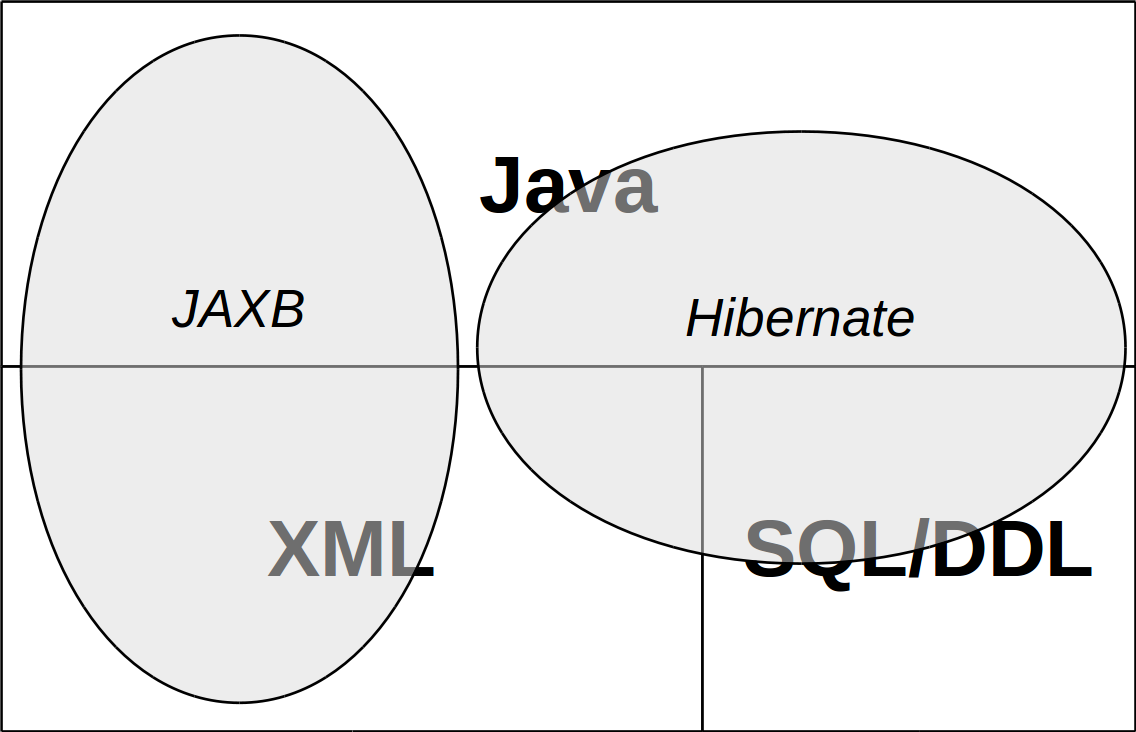
\includegraphics[width=.6\textwidth]{images/JORXDomains.png}
\end{center}
{
\scriptsize 
This schematic illustration depicts the interrelation among linguistic domains of example corpus used.
It depicts languages and technologies for \gls{O/R/X-Mapping} with \gls{Java}.
}
\caption{Example Corpus Domains: Java O/R/X}
\label{figure:ExampleCorpusJORXDomains}
\end{figure}

The languages (\gls{Java}, \gls{XML} \& \gls{SQL}) in Figure \ref{figure:ExampleCorpusJORXDomains} are displayed as disjoint square sets.
Technologies (\gls{JAXB} \& \gls{Hibernate}) are displayed as oval sets intersecting languages.
This is due to their linguistic nature, e.g. \gls{JAXB} produces specific \Gls{Java}- and \gls{XML}-Code which does not necessarily intersect with code produced by other technologies.
\gls{Hibernate} intersects all three languages.
It uses \gls{XML} files or \gls{Java}-Annotations for describing \gls{O/R-Mapping} of a data-model and generates \gls{SQL} artifacts according to that mapping.
In this sense, technologies create technology-specific subsets of a languages.

\section{Setup}
\label{section:Setup}
The implemented recovery system is evaluated with the \gls{Megamodel} shown in listing \ref{listing:EvaluatedMegamodel}.
\begin{lstlisting}[
caption={Megamodel Setup},
label={listing:EvaluatedMegamodel}]
companyJavaFile : File
companyJavaFile = 'workspace:/org.softlang.megal.plugins/input/Company.java'

companyHbmFile : File
companyHbmFile = 'workspace:/org.softlang.megal.plugins/input/Company.hbm.xml'

departmentJavaFile : File
departmentJavaFile = 'workspace:/org.softlang.megal.plugins/input/Department.java'

departmentHbmFile : File
departmentHbmFile = 'workspace:/org.softlang.megal.plugins/input/Department.hbm.xml'

employeeJavaFile : File
employeeJavaFile = 'workspace:/org.softlang.megal.plugins/input/Employee.java'

employeeHbmFile : File
employeeHbmFile = 'workspace:/org.softlang.megal.plugins/input/Employee.hbm.xml'

companiesXmlFile: File
companiesXmlFile = 'workspace:/org.softlang.megal.plugins/input/companies.xml'

companiesXsdFile: File
companiesXsdFile = 'workspace:/org.softlang.megal.plugins/input/companies.xsd'

comaniesSqlFile : File
comaniesSqlFile = 'workspace:/org.softlang.megal.plugins/input/companies.ddl.sql'

companyJavaFile correspondsTo companiesXsdFile
companyJavaFile correspondsTo comaniesSqlFile
companyJavaFile correspondsTo companyHbmFile

departmentJavaFile correspondsTo companiesXsdFile
departmentJavaFile correspondsTo comaniesSqlFile
departmentJavaFile correspondsTo departmentHbmFile

employeeJavaFile correspondsTo companiesXsdFile
employeeJavaFile correspondsTo comaniesSqlFile
employeeJavaFile correspondsTo employeeHbmFile

companiesXmlFile conformsTo companiesXsdFile
\end{lstlisting}
We declare nine \glspl{Artifact} to be files and bind them to locations on the local file system.
For each class of the \gls{101HRMS} model, i.e. company, department and employee, we declare a pair of entities comprising a \gls{Java} class file and a \gls{Hibernate} mapping file.
For the \gls{101HRMS} model at whole, \glspl{Artifact} for its \gls{XML}, \gls{XSD} and \gls{SQL/DDL} representations are declared.
Following this, we declare the expected \gls{Correspondence} and \gls{Conformance} relations among the files.

\section{Metrics}
\label{section:Metrics}
We evaluate the implemented recovery system regarding the requirements stated in §\ref{section:Requirements}, i.e. requirements \ref{requirement:FragmentRecovery}, \ref{requirement:ParthoodRecovery}, \ref{requirement:CorrespondenceRecovery} and \ref{requirement:ConformanceRecovery} for recovery of \gls{Parthood}, \glspl{Fragment}, \gls{Correspondence} links and \gls{Conformance} links.

For this, we measure the quantity of all entities of concern grouped by type, i.e. \glspl{Artifact}, files and \glspl{Fragment}:
\begin{align*}
\#\Artifact &:= |\{ x : \Artifact(x) \}| \\
\#\File &:= |\{ x : \File(x) \}| \\
\#\Fragment &:= |\{ x : \Fragment(x) \}|
\end{align*}
We also measure the overall amount of all relevant links grouped by type, i.e.
\partOf, \fragmentOf, \correspondsTo~ and \conformsTo:
\begin{align*}
\#\partOf &:= |\{ (x,y) : \partOf(x,y) \}| \\
\#\fragmentOf &:= |\{ (x,y) : \fragmentOf(x,y) \}| \\
\#\correspondsTo &:= |\{ (x,y) : \correspondsTo(x,y) \}| \\
\#\conformsTo &:= |\{ (x,y) : \conformsTo(x,y) \}| 
\end{align*}

For a more differentiated look on requirements \ref{requirement:FragmentRecovery} and \ref{requirement:ParthoodRecovery}, we measure the number of parts and \glspl{Fragment} of a specific entity:
\begin{align*}
\#\partOf(x) &:= |\{ y : \partOf(y,x) \}| \\
\#\fragmentOf(x) &:= |\{ y : \fragmentOf(y,x) \}| 
\end{align*}

For requirements \ref{requirement:CorrespondenceRecovery} and \ref{requirement:ConformanceRecovery}, i.e. \gls{Correspondence} and \gls{Conformance} recovery, we devise a similar measurement.
However, we do not count the number of entities corresponding or conforming to a given other entity.
We rather count entities corresponding or conforming to \glspl{Fragment} of the given entity.
\begin{align*}
\#\correspondsTo(y) &:=
|\{ x : \correspondsTo(x,y') \wedge \fragmentOf(y',y)  \}|
\\
\#\conformsTo(y) &:=
|\{ x : \conformsTo(x,y') \wedge \fragmentOf(y',y)  \}|
\end{align*}

Eventually, we are interested in the number of unique elements per relationship, distinguishing left-hand side (LHS) from right-hand side (RHS) entities: 
\begin{align*}
\#LHS(R) &:= |\{ x : R(x,y) \}| \\
\#RHS(R) &:= |\{ y : R(x,y) \}| 
\end{align*}

\section{Results}
\label{section:Results}
An evaluation of the setup described in §\ref{section:Setup} with the metrics of §\ref{section:Metrics} provides the following results.
Table \ref{table:NumberOfRecoveredArtifactsFilesAndFragments} shows the number of all \glspl{Artifact}, files and \glspl{Fragment} in the \gls{Megamodel} after execution.
\begin{table}[h!]
\begin{center}
\begin{tabular}{|l|l|l|}
\hline
$\#\Artifact$ & $\#\File$ & $\#\Fragment$
\\ \hline
483 & 9 & 474 
\\ \hline
\end{tabular}
\end{center}
\caption{Number of recovered artifacts, files and fragments}
\label{table:NumberOfRecoveredArtifactsFilesAndFragments}
\end{table}
It indicates that files and \glspl{Fragment} are disjoint as proposed by axiom \ref{axiom:Fragment} in §\ref{section:AxiomsOfLinguisticArchitectures}.
All files and all fragments are artifacts, so their numbers sum up to the number of artifacts: $\#\Artifact = \#\File + \#\Fragment$.
The number of files matches the given setup (see §\ref{section:Setup}); the remaining \glspl{Artifact} are \glspl{Fragment}.

Table \ref{table:NumberOfRecoveredParthoodFragmentCorrespondenceAndConformanceLinks} shows the number of recovered \glspl{TraceLink} for \gls{Parthood}, \gls{Fragment}, \gls{Correspondence} and \gls{Conformance} relations.
\begin{table}[h!]
\begin{center}
\begin{tabular}{|l|l|l|l|}
\hline
$\#\partOf$ & $\#\fragmentOf$ & $\#\correspondsTo$ & $\#\conformsTo$
\\ \hline
1847 & 1837 & 106 & 81 
\\ \hline
\end{tabular}
\end{center}
\caption{Number of recovered parthood, fragment, correspondence and conformance links}
\label{table:NumberOfRecoveredParthoodFragmentCorrespondenceAndConformanceLinks}
\end{table}
The numbers for \partOf- and \fragmentOf- relationships do not match.
This can be explained with the usage of \partOf~ to configure plug-ins by \gls{MegaL/Xtext} \cite{LukasHaertelBScThesis}.
Moreover, the numbers for \gls{Parthood} and \gls{Fragment} links are relatively large compared to the overall number of \glspl{Artifact} in table \ref{table:NumberOfRecoveredArtifactsFilesAndFragments}.
This may be due to the simplicity of the metric.
It simply counts all unique pairs.
\Gls{Parthood} and \gls{Fragment} links are transitive, which leads to this accumulation.

On the other hand, the number of recovered \gls{Correspondence} and \gls{Conformance} links are relatively small compared to the number of \Gls{Parthood} and \gls{Fragment} links.
This can be explained by the nature of the recovery method in conjunction with the setup.
\gls{Java} classes and the majority of classical object-oriented programming languages group behavior and structure.
A class may contain field- and method-\glspl{Fragment}, which are also recovered.
However, only the former may be linked through \gls{Correspondence} and \gls{Conformance} within the given setup.

Table \ref{table:NumberOfPartsAndFragmentsPerFile} shows the number of recovered parts and \glspl{Fragment} per file. 
\begin{table}[h!]
\begin{center}
\begin{tabular}{|l|l|l|}
\hline
$x$ & $\#\partOf(x)$ & $\#\fragmentOf(x)$
\\ \hline
companyJavaFile & 9 & 9 
\\ \hline
companyHbmFile & 51 & 51 
\\ \hline
departmentJavaFile & 20 & 20 
\\ \hline
departmentHbmFile & 112 & 112 
\\ \hline
employeeJavaFile & 15 & 15 
\\ \hline
employeeHbmFile & 76 & 76 
\\ \hline
companiesXmlFile & 89 & 89 
\\ \hline
companiesXsdFile & 85 & 85 
\\ \hline
comaniesSqlFile & 17 & 17 
\\ \hline \hline
\textbf{Sum:} & 474 & 474 
\\ \hline 
\end{tabular}
\end{center}
\caption{Number of parts and fragments per file}
\label{table:NumberOfPartsAndFragmentsPerFile}
\end{table}
The overall equivalence $\#\partOf(x) = \#\fragmentOf(x)$ for all files indicates that all parts of each file are indeed proper parts (see §\ref{subsection:Fragments}).
Furthermore it indicates in conjunction with table \ref{table:NumberOfRecoveredArtifactsFilesAndFragments} that all recovered \glspl{Fragment} are properly linked to the files their originated from, since sum of all recovered \glspl{Fragment} per file matches the number of all recovered \glspl{Fragment}.

Table \ref{table:NumberOfEntitiesCorrespondingOrConformingToFragmentsOfAFile} shows the number of entities corresponding of conforming to \glspl{Fragment} of a file.
\begin{table}[h!]
\begin{center}
\begin{tabular}{|l|l|l|}
\hline
$x$ & $\#\correspondsTo(x)$ & $\#\conformsTo(x)$
\\ \hline
companyJavaFile & 12 & 0 
\\ \hline
companyHbmFile & 4 & 0 
\\ \hline
departmentJavaFile & 15 & 0 
\\ \hline
departmentHbmFile & 5 & 0 
\\ \hline
employeeJavaFile & 17 & 0 
\\ \hline
employeeHbmFile & 5 & 0 
\\ \hline
companiesXmlFile & 0 & 0 
\\ \hline
companiesXsdFile & 16 & 67 
\\ \hline
comaniesSqlFile & 11 & 0 
\\ \hline 
\end{tabular}
\end{center}
\caption{Number of entities corresponding or conforming to fragments of a file}
\label{table:NumberOfEntitiesCorrespondingOrConformingToFragmentsOfAFile}
\end{table}
For instance the twelve entities corresponding to a fragment of companyJavaFile are shown in listing \ref{listing:RecoveredCorrespondences}, which shows that all \gls{Java} fields are linked to corresponding \gls{XSD} attribute declarations, \gls{Hibernate} mapping declarations or \gls{SQL/DDL} column declarations, except for fields implying a foreign key relationship.
\begin{lstlisting}[caption={Recovered Correspondences},label={listing:RecoveredCorrespondences}]
comaniesSqlFile.F3$Company correspondsTo companyJavaFile.Company
comaniesSqlFile.F3$Company.F0$name correspondsTo companyJavaFile.Company.F5$name
comaniesSqlFile.F3$Company.F1$id correspondsTo companyJavaFile.Company.F6$id

companiesXsdFile.F0$xs:schema.F2$xs:element correspondsTo companyJavaFile.Company
companiesXsdFile.F0$xs:schema.F5$xs:complexType correspondsTo companyJavaFile.Company
companiesXsdFile.F0$xs:schema.F5$xs:complexType.F2$xs:attribute correspondsTo companyJavaFile.Company.F6$id
companiesXsdFile.F0$xs:schema.F5$xs:complexType.F3$xs:attribute correspondsTo companyJavaFile.Company.F5$name
companiesXsdFile.F0$xs:schema.F5$xs:complexType.F1$xs:sequence.F0$xs:element correspondsTo companyJavaFile.Company.F4$departments

companyHbmFile.F0$hibernate-mapping.F4$class correspondsTo companyJavaFile.Company
companyHbmFile.F0$hibernate-mapping.F4$class.F10$property correspondsTo companyJavaFile.Company.F5$name
companyHbmFile.F0$hibernate-mapping.F4$class.F8$id correspondsTo companyJavaFile.Company.F6$id
companyHbmFile.F0$hibernate-mapping.F4$class.F9$bag correspondsTo companyJavaFile.Company.F4$departments
\end{lstlisting}

$\#\correspondsTo(\text{companiesXmlFile}) = 0$ indicates that \gls{Correspondence} does not occur between model- and instance-level \glspl{Artifact}.
This satisfies the definition of \gls{Correspondence}, denoting two \glspl{Artifact} represent the same data (see §\ref{subsection:Correspondence}), which should not occur between different levels of abstraction.

Regarding \gls{Conformance}, the table indicates, that it only occurs towards \gls{XSD} files, since $\#\conformsTo(x)$ is zero for all files except companiesXsdFile.
This is in accordance with the definition of \gls{Conformance}, given within the setup \gls{XSD} is the only specification \gls{Language} for the other \glspl{Artifact} present.

Table \ref{table:NumberOfUniqueEntitiesPerRelationship} shows the number of unique entities per relationship.
We distinguish left-hand side (LHS) from right-hand side (RHS) entities.
\begin{table}[h!]
\begin{center}
\begin{tabular}{|l|l|l|}
\hline
$R$ & $\#LHS(R)$ & $\#RHS(R)$
\\ \hline
$\partOf$ & 484 & 121
\\ \hline
$\fragmentOf$ & 474 & 117
\\ \hline
$\correspondsTo$ & 68 & 68
\\ \hline
$\conformsTo$ & 68 & 19
\\ \hline 
\end{tabular}
\end{center}
\caption{Number of unique entities per relationship}
\label{table:NumberOfUniqueEntitiesPerRelationship}
\end{table}
The number of corresponding and conforming entities is significantly lower than the overall number of recovered \glspl{Fragment} in table \ref{table:NumberOfRecoveredArtifactsFilesAndFragments}.
This may indicate recovery of unnecessary \glspl{Fragment}, e.g. \glspl{Java} method \glspl{Fragment}; or it indicates an insufficiency of the implemented \gls{Correspondence} and \gls{Conformance} recovery.
However, the number of unique left-hand side entities for \conformsTo~ matches the number of $\#\conformsTo(\text{companiesXsdFile})$ minus one, the latter being the initial \conformsTo-declaration from the setup (see §\ref{section:Setup}).
This assures that \gls{Conformance} is only recovered towards \gls{XSD}.
Likewise the number of unique left-hand side entities for \fragmentOf~ matches the number of all recovered \glspl{Fragment} from table \ref{table:NumberOfRecoveredArtifactsFilesAndFragments}, the delta to \partOf~ remaining the same for both sides.